\chapter{Rubrik nivå 1}
Sidorna i huvuddelen numreras löpande med början på 1. De sidor som föregår
huvuddelen (sammanfattning och innehållsförteckning) numreras separat med
romerska siffror. 

\section{Rubrik nivå 2}
I föreliggande rapportmall används huvudsakligen teckensnittet
\textit{Garamond} för löpande text och \textit{Arial} för rubriker. För
symboler som konstanter och variabler skall teckensnittet \textit{Cambria}
användas, såväl i ekvationer som när de skrivs i den löpande texten. För
grekiska tecken används teckensnittet \textit{Symbol}. För listning av
programkod eller liknande rekommenderas att ett teckensnitt med fast
teckenbredd används, exempelvis \textit{Courier}.

\subsection{Rubrik nivå 3}
I mallen finns formatmallar för stycken av olika typ, exempelvis används
formatmallen \textit{Brödtext} (eng: \textit{Body Text}) för alla stycken
som är löpande text och \textit{Rubrik 1}, \textit{Rubrik 2}, ... (eng:
\textit{Heading 1}, \textit{Heading 2}, ...) för rubriker på olika nivåer.

Följande stycke är ett så kallat blockcitat formaterat som \textit{Citat}
(eng: \textit{Quote}):

\begin{displayquote}
    There is an art to flying, or rather a knack. Its knack lies in learning
    to throw yourself at the ground and miss. ... Clearly, it is this
    second part, the missing, that presents the difficulties. (Adams, 1982)
\end{displayquote}

Nedan följer exempel där formatmallen \textit{Beskrivning} (eng:
\textit{Caption}) används på förklaringarna till \ref{tab:fruits} och 
\ref{fig:flowchart}. I \LaTeX finns även möjlighet att infoga automatisk
numrering och hänvisning genom att använda \verb|\ref| och \verb|\label|.

\begin{table}[ht!]
    \label{tab:fruits}
    \centering
    \caption{Två olika frukters egenskaper.}
    \begin{tabular}{|l|l|l|l|}
        \hline
        & \textbf{Form} & \textbf{Färg} & \textbf{Smak} \\
        \hline
        \textbf{Banan} & Långsmal & Gul & Söt \\
        \hline
        \textbf{Citron} & Rund & Gul & Sur \\
        \hline
    \end{tabular}
\end{table}

\begin{figure}[ht!]
    \label{fig:flowchart}
    \centering
    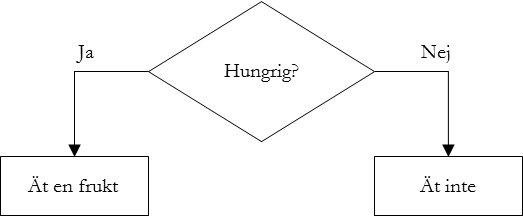
\includegraphics[width=7cm]{images/flowchart}
    \caption{Ett enkelt flödesschema}
\end{figure}

\subsubsection{Rubrik nivå 4}
I mallen är avsnitt på nivå 4 numrerade, men numreringen med fyra nummer
kan i många fall upplevas som förvillande och bör normalt undvikas. Det
rekommenderas att istället använda formatmallen \textit{Rubrik 5} (eng:
\textit{Heading 5}) på dessa rubriker, se följande avsnittsrubrik. 

\paragraph{Rubrik nivå 5}
För att ekvationer ska få rätt utseende och samtidigt kunna numreras används
miljön \verb|equation|. \LaTeX formatterar automatiskt så ekvationen
centreras och numreras. 

\begin{equation}
    \label{eq:integral}
    I_0 = \frac{1}{T}\int_0^T i(t)dt
\end{equation}

I kontrast till Microsoft Word behövs här inga tabeller för formatteringen
och numreringen utan \LaTeX har inbyggt stöd. Vill man ha en ekvation
utan numrering kan man använda miljön \verb|align*|. 

\begin{align*}
    e^{i\pi}-1=0
\end{align*}

\LaTeX hanterar numreringen automatiskt och för att referera till en
ekvation kan man lägga in \verb|label| och använda \verb|\ref| som detta:
\ref{eq:integral}. 
